\chapter{Analysis}

\section{Introduction}

\subsection{Client Identification} 
My client is Tom Wolf. He is employed as a teacher at Long Road Sixth Form College. He teaches A level ICT, Diploma ICT and GCSE ICT. I deliberately chose Tom to give me a project for A level Computing as he is my ICT teacher and therefore I usually see him at least 3 times a week and if I will require additional information then this should not be a problem. Also, if I will require additional information for this project, then I could use the school email to request more information from Tom. 
 
\subsection{Define the current system} 
In the current system, Tom has to set an assignment for the students, this can be a test, homework or coursework. After the assignment is completed by students, Tom then has to mark the assignment. Based on the maximum possible mark and achieved mark, Tom calculates the grade using a specific algorithim. Then using google drive, Tom creates a spreadsheet and inserts all of the grades. After several assignments, Tom then calculates the end of unit predicted grade (using a specific algorithm). Usually a unit is a school term or a topic (if multiple topics are covered in one term). After several units, Tom then calculates the end of the year predicted grade (using a specific algorithm). All of the predicted grades are inserted into the google drive database and stored. This way Tom can access his spreadsheet on his mobile (LG G3) anywhere as long as he has access to internet or his laptop or his iPad 2. 

\subsection{Section appendix}

What system do you use currently?
- I use an iPad, LG G3 mobile, mid range school laptop and a very old home desktop to access my google drive spread sheets in which I store my students' grades and predicted grades, which I have to calculate myself.

Is there anything in the current system that could be improved?
- I must calculate all of the grades, end of the unit predicted grades, end of the year predicted grades separately for all of the students. Then I need to insert all of that into the google drive database. And I need to do this very frequently, at least twice a term for every class that I have, which on average consists of 18 students. 

How should the data be stored in the system?
-Throughough the year, there are few units, those units usually are school terms and within the school units are assignments, which represent all of the work which I grade myself. I should be able to add as many as possible assignments into each unit, although the amount of units could be permenantly fixed. Preferably I should be able to add and delete units based on my requirements.

\subsection{Describe the problems}

Tom is required to calculate predicted grades for 100 students by himself and this requires his own time, so the school does not pay him for this. So, for Tom this is not satisfactory as 100 students is a big amount and so it requires a lot of effort and time. Therefore, Tom requires a system that will perform those calculations automatically. 

\section{Investigation}

\subsection{The current system}
\subsubsection{Data sources and destinations}

In the current system, the main source of data are the students, from which Tom 
takes their first name and last name. Assignments, from which Tom is able to calculate grades and T

\begin{center}
    \begin{tabular}{|p{4cm}|p{4cm}|p{4cm}|p{4cm}}
        \hline
        \textbf{Data Source} & \textbf{data} & \textbf{Travels via} &  \textbf{Destination} \\ \hline
Students & First Name, Last Name & Written, Email & Teacher(Tom) \\
\hline
Tom & Grades, Predicted Grades, Achieved Mark, Achieved Percentage & Written, Verbal, Email & Students \\
\hline
Assignments & Grades & Written, Email & Tom/Databse \\ 
\hline
\end{tabular}
\end{center}



\subsubsection{Algorithms}

\begin{algorithm}[H]
\label{}
    \caption{End of the unit predicted grade}
\begin{algorithmic}[1]
\SET{$Score$}{$0$}
\For{$grade$}{$Assignment$}
     \If{$grade = "A*"$}
          \SET{$Score$}{$Score+6$}
     \ElsIf{$grade = "A"$}
          \SET{$Score$}{$Score+5$}
     \ElsIf{$grade = "B"$}
          \SET{$Score$}{$Score+4$}
     \ElsIf{$grade = "C"$}
          \SET{$Score$}{$Score+3$}
     \ElsIf{$grade = "D"$}
          \SET{$Score$}{$Score+2$}
     \ElsIf{$grade = "E"$}
          \SET{$Score$}{$Score+1$}
     \EndIf
\EndFor
\SET{$Score$}{$Score / length(assignments)$}

\If{$Score > 5.5$}
     \SET{$Score$}{$EndOfUnitG = "A*"$}
\ElsIf{$Score > 4.5$}
     \SET{$Score$}{$EndOfUnitG = "A"$}
\ElsIf{$Score > 3.5$}
     \SET{$Score$}{$EndOfUnitG = "B"$}
\ElsIf{$Score > 2.5$}
     \SET{$Score$}{$EndOfUnitG = "C"$}
\ElsIf{$Score > 1.5$}
     \SET{$Score$}{$EndOfUnitG = "D"$}
\ElsIf{$Score > 0.5$}
     \SET{$Score$}{$EndOfUnitG = "E"$}
\Else
     \SET{$Score$}{$EndOfUnitG = "U"$}
\EndIf
\end{algorithmic}
\end{algorithm}

\begin{algorithm}[H]
\label{}
    \caption{End of the year predicted grade(for AS)}
\begin{algorithmic}[1]
\For{$grade$}{$Unit$}
     \If{$grade = "A*"$}
          \SET{$Score$}{$Score+6$}
     \ElsIf{$grade = "A"$}
          \SET{$Score$}{$Score+5$}
     \ElsIf{$grade = "B"$}
          \SET{$Score$}{$Score+4$}
     \ElsIf{$grade = "C"$}
          \SET{$Score$}{$Score+3$}
     \ElsIf{$grade = "D"$}
          \SET{$Score$}{$Score+2$}
     \ElsIf{$grade = "E"$}
          \SET{$Score$}{$Score+1$}
     \EndIf
\EndFor
\SET{$Score$}{$Score / length(units)$}
\end{algorithmic}
\end{algorithm}

\begin{algorithm}[H]
\label{}
    \caption{}
\begin{algorithmic}[1]

\If{$Score > 5.5$}
     \SET{$Score$}{$ASPredictedG = "A*"$}
\ElsIf{$Score > 4.5$}
     \SET{$Score$}{$ASPredictedG = "A"$}
\ElsIf{$Score > 3.5$}
     \SET{$Score$}{$ASPredictedG = "B"$}
\ElsIf{$Score > 2.5$}
     \SET{$Score$}{$ASPredictedG = "C"$}
\ElsIf{$Score > 1.5$}
     \SET{$Score$}{$ASPredictedG = "D"$}
\ElsIf{$Score > 0.5$}
     \SET{$Score$}{$ASPredictedG = "E"$}
\Else
     \SET{$Score$}{$ASPredictedG = "U"$}
\EndIf
\end{algorithmic}
\end{algorithm}


\begin{algorithm}[H]
\label{}
    \caption{Calculating the grade}
\begin{algorithmic}[1]
\SET{$percent$}{$(AchievedMark / MaxMark) * 100$}
\If{$percent > "90"$}
       \SET{$grade$}{$A*$}
\ElsIf{$percent = "80"$}
       \SET{$grade$}{$A$}
\ElsIf{$percent = "70"$}
       \SET{$grade$}{$B$}
\ElsIf{$percent = "60"$}
       \SET{$grade$}{$C$}
\ElsIf{$percent = "50"$}
       \SET{$grade$}{$D$}
\ElsIf{$percent = "40"$}
       \SET{$grade$}{$E$}
\Else
       \SET{$grade$}{$U$}
\EndIf
\end{algorithmic}
\end{algorithm}

\subsubsection{Data flow diagram}

\begin{figure}[H]
    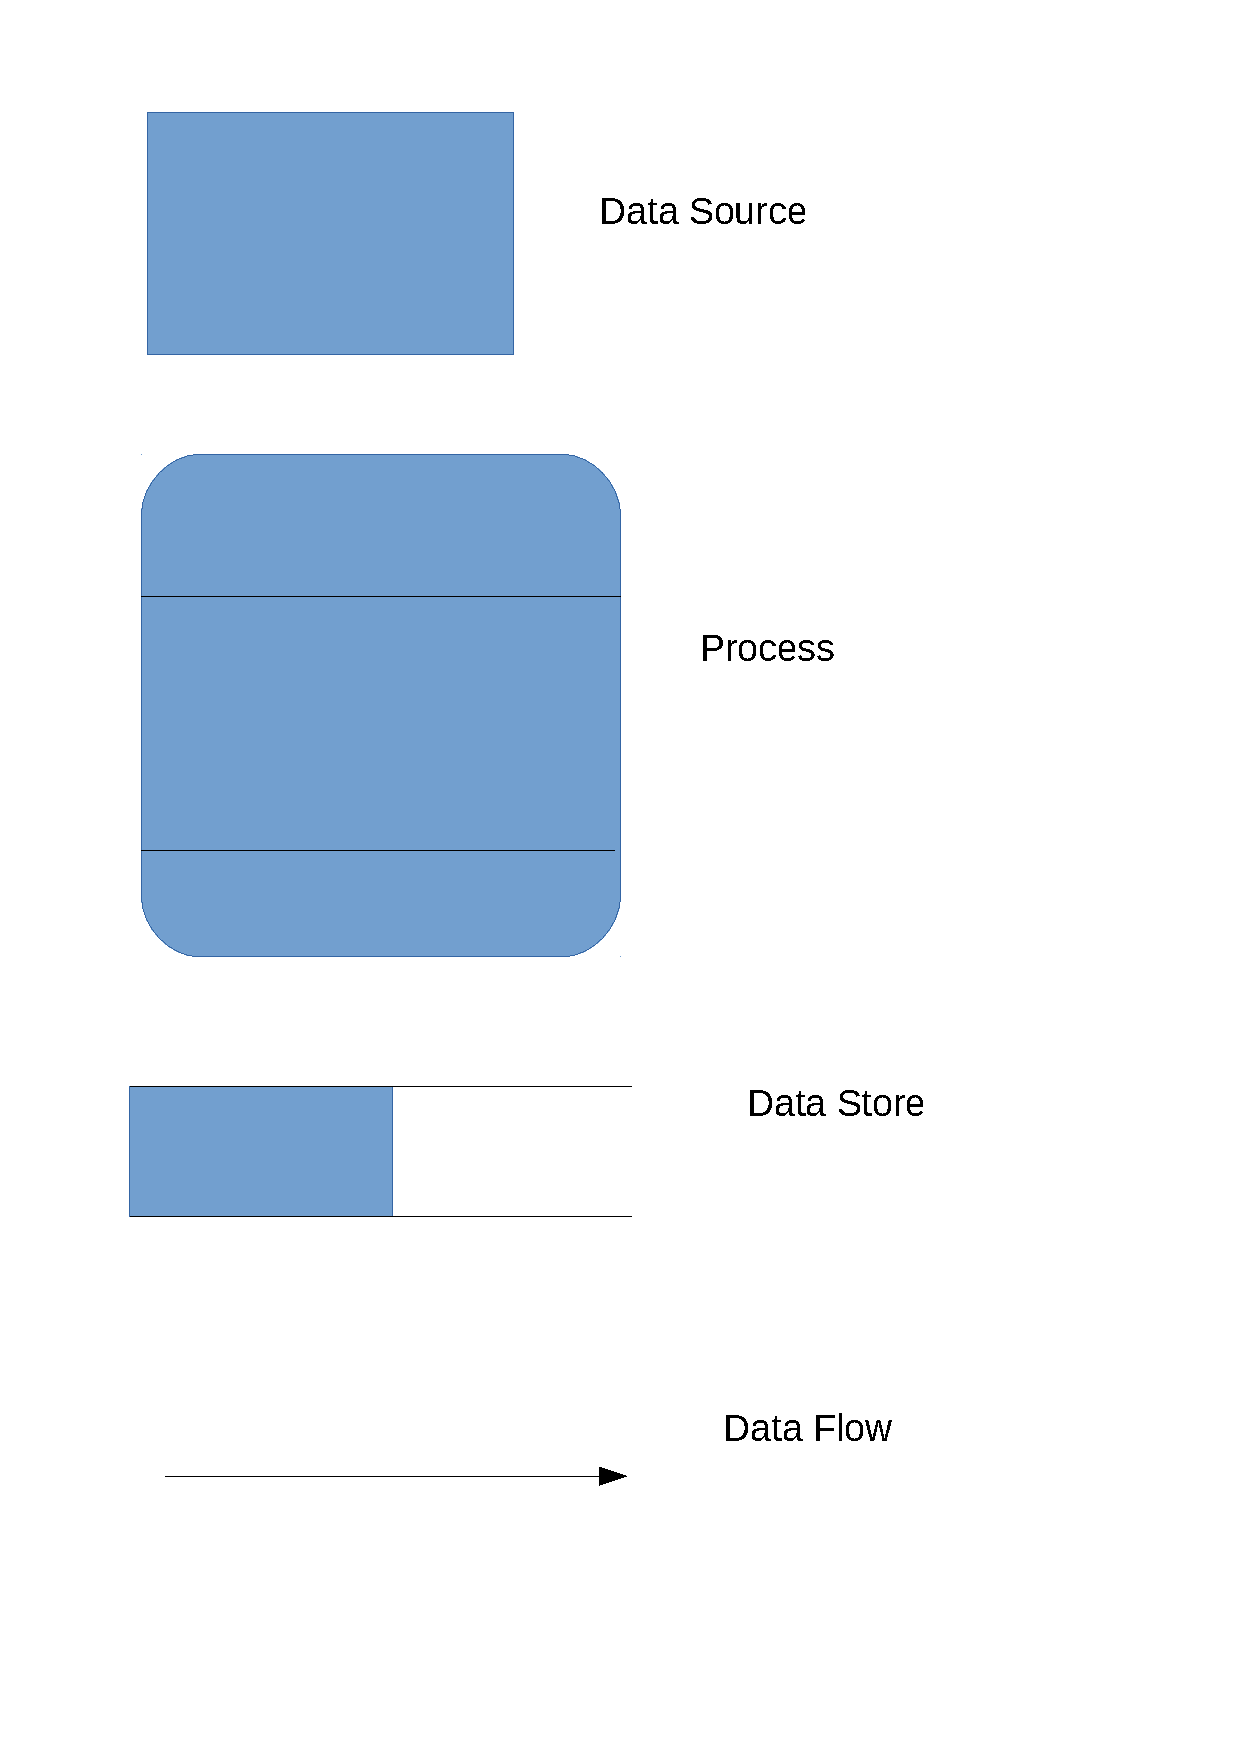
\includegraphics[width=\textwidth]{./Analysis/images/key.pdf}
\end{figure} 

\begin{figure}[H]
    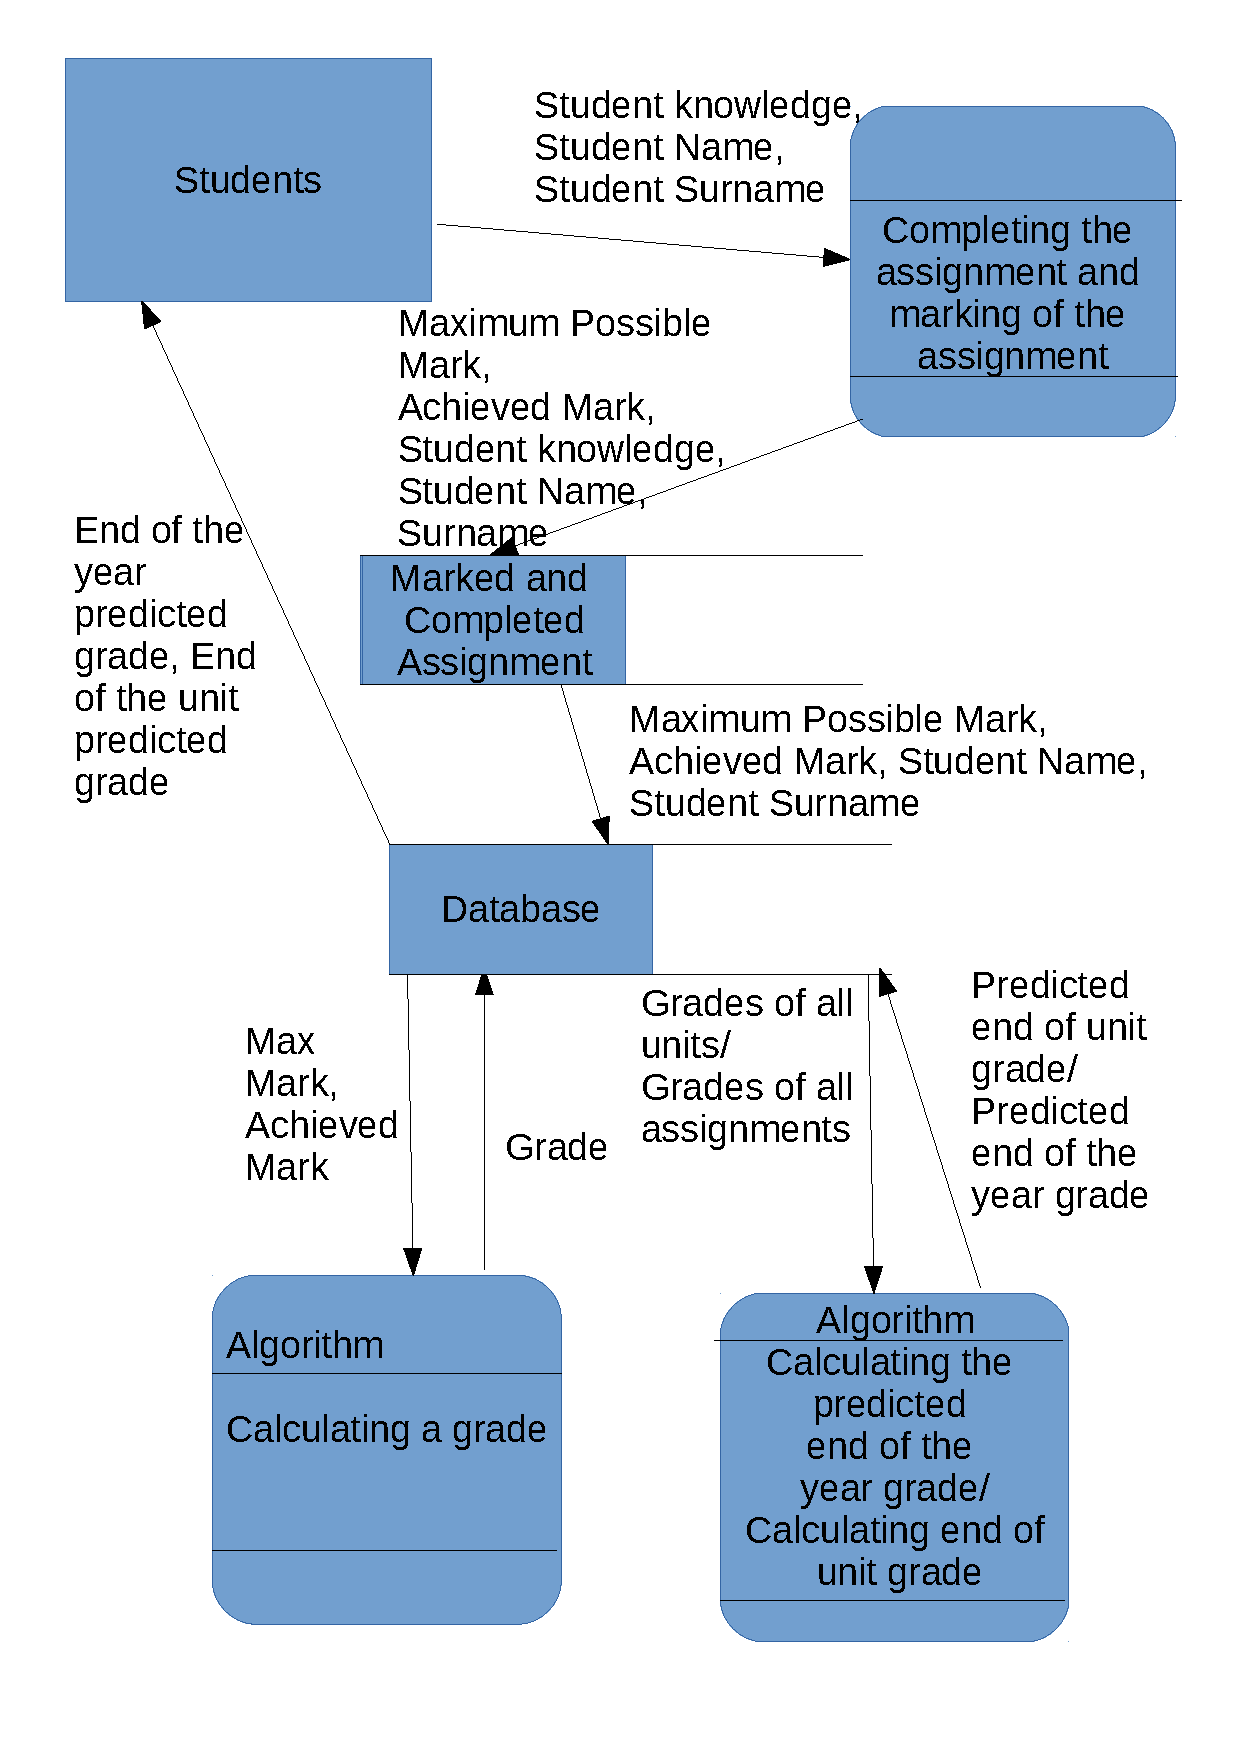
\includegraphics[width=\textwidth]{./Analysis/images/222DataFlowDiagram.pdf}
\end{figure}

\subsubsection{Input Forms, Output Forms, Report Formats}

In the current system, the main input form are the assignments, which are used by students to complete a task set by Tom. Students using their knowledge complete the assignments. This can be done either electronically by students or on paper (which in some cases is the only option, such as an end of unit test). After the assignment is completed, Tom then marks the paper and that is how Tom gets the achieved unit mark. 

There are several output formats. If the assignment was done electronically, then Tom usually sends an email back to the student with the achieved mark and grade with comments on what can be improved. If the assignment was done on paper, then Tom writes on the paper where are the errors and what is missing, as well as the achieved mark and achieved grade.

Another output format is Tom either speaking to every student individually or to the whole class as a whole.

\subsection{The proposed system}
\subsubsection{Data flow diagram}

The data flow diagram in the proposed system is exactly the same in the current in the current system, the only difference is that the elgorithms are going to be performed by the new system electronically, whereas in the current system all algorithms are performed by Tom manually.

\begin{figure}[H]
    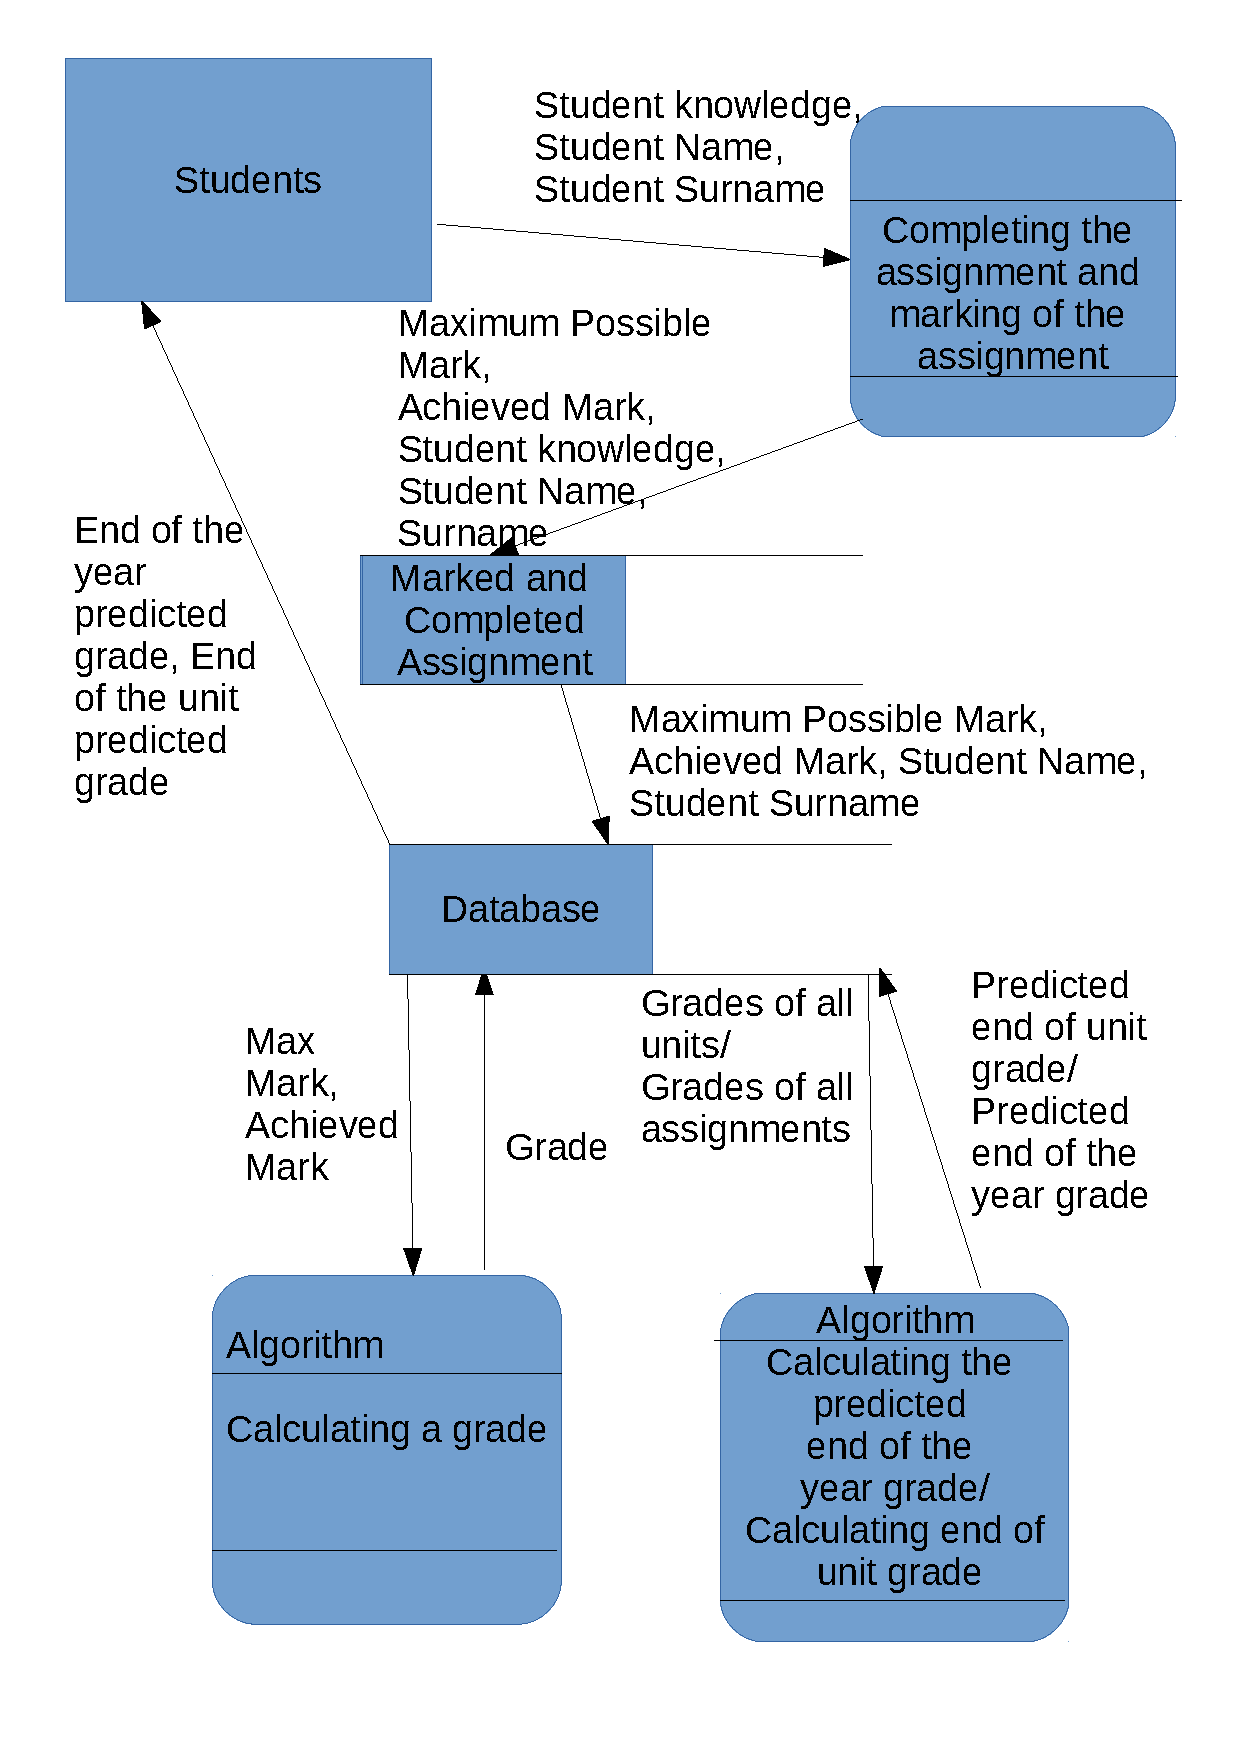
\includegraphics[width=\textwidth]{./Analysis/images/222DataFlowDiagram.pdf}
\end{figure}

\subsubsection{Data dictionary}
\begin{center}
    \begin{tabular}{|p{2cm}|p{2cm}|p{2cm}|p{2cm}|p{2cm}}
        \hline
        \textbf{Name} & \textbf{Data Type} & \textbf{Length} &  \textbf{Validation} & \textbf{Examples} \\
StudentID & Integer & 1-600 & Range & 60,1,600 \\
\hline
StudentName & String & 3-25 Characters & Length & Mateusz \\
\hline
StudentSurn & String & 3-30 Characters & Length & Parfienczyk \\
\hline
StudentEmail & String & 5-40 Characters & Length & example@ longroad.ac.uk \\
\hline
MaxMark & Integer & 1-1000 & Range & 200,475 \\
\hline
AchievedMark & Integer & 0-1000 & Range, cannot be bigger than MaxMark for the same & assignment 250,400,300 \\
\hline
Mark Percentage & Integer & 0-100 & Range & 30,50,73 \\
\hline
Assignment Completed & Boolean & Presence Check & True, False \\
\hline
UnitPredicted G & String & 1 Character & Length & A,B,C,D,E,U \\
\hline
ASPredictedG & String & 1 Character & Length & A,B,C,D,E,U \\
\hline
EndOfUnitG & String & 1 Character & Length & A,B,C,D,E,U \\
ASGrade & String & 1 Character & Length & A,B,C,D,E,U \\
\hline
A2PredictedG & String & 1 Character & Length & A,B,C,D,E,U \\
\hline
\end{tabular}
\end{center}


\subsubsection{Volumetrics}

\section{Objectives}

\subsection{General Objectives}
The program must have a database separately from the main file, so that Tom could use a tool such as Google Drive to store just the data file for backup or so that he could download and view the data on different computers as long as he will have access to internet.

\subsection{Specific Objectives}
The system must be simple and easy to use with readable text and simple font, so that Tom would be able to read text without frustration and access his data quickly. 

The database must allow Tom to alter grades and predicted grades because he has privilages to do so as a teacher.

\subsection{Core Objectives}
The system should be as responsive as possible, the system should be able to calculate grades as quickly as possible as well as save data to database, so that Tom could save as much time as possible

\subsection{Other Objectives}
The system should allow Tom to view data from the database in a table format, which Tom will be able to customise himself and it also should be appealing to Tom, so that use of the system would be satisfying.

\section{ER Diagrams and Descriptions}

\subsection{ER Diagram}

\subsection{Entity Descriptions}

\section{Object Analysis}

\subsection{Object Listing}

\begin{enumerate}
    \item Teacher
    \item Student
    \item Assignment
\end{enumerate}

\subsection{Relationship diagrams}

\subsection{Class definitions}

\section{Other Abstractions and Graphs}

\section{Constraints}
\subsection{Hardware}
Tom current mostly uses his college laptop for any computer work with Windows 7 64 bit operating system and 15.4" display.Tom also has a LG G3 mobile phone with a 5.5" display and Android 4.4.2 "KitKat" operating system and an iPad 2 with 9.7" display with iOS 8.1 operating system.

\subsection{Software}
Tom would like the software to be compatible with his iPad 2 operating system (iOS) or his LG G3 operating system (Android 4.4.2 "KitKat"), although this is not a must as long as it is going to function quickly and correctly on his school laptop (Windows 7 64-bit operating system).

\subsection{Time}
The very final deadline for this whole project is Friday, 1 May 2015, which is set by Adam, although the implementation deadline is Friday 13th February.
Tom does not have any preference when the system should be finished because the current system is satisfactory and the earliest he would prefer to switch to the new system would be next school year (September 2015).

\subsection{User Knowledge}
Since Tom is an ICT teacher, his knowledge about computers is very high, but his programming knowledge is poor and this is why he has not made an electronic markook himself for his requirements. He is more than capable of using a computer and complicated computer applications, so Tom should not have a difficulty using the electronic markbook once it is going to be finished.

\subsection{Access restrictions}
The database should only be accessed by Tom. The database should be protected with a password so that no one could access the database and alter the data, such as students which would want to change their assignment grades or predicted grades.

\section{Limitations}

\subsection{Areas which will not be included in computerisation}
All of the marking has to be done by Tom, entering the mark also has to be done by Tom.

\subsection{Areas considered for future computerisation}
The student names, surnames and emails could possibly be imported from the school database/network. Also, the grades and predicted grades could be sent automatically with a capable of doing this system.

\section{Solutions}

\subsection{Alternative solutions}
Web based application - Tom would be able to access his data as long as he would have internet access and he would not need to have the system installed on his device as the system would be installed on internet. The down side is that this is very challenging to complete and also the data would be exposed to hackers and thiefs if the data will not be secured correctly (and this also can be quite challenging).  

\subsection{Justification of chosen solution}
To complete this project, I will use Python and PyQT python extension/module because I learned the basics of Python in AS computing and I am continuing computing this year, so my Python programming skills will also improve throughout the year and they will help me with this task. Additionally, my teacher Adam McNicol strongly recommended Python for the whole class and in the past when I had issues or could not understand Python, most of the time Adam McNicol was able to help me resolve any issue. So if I am going to have issues with Python when coding the system, hopefully Adam will be able to help me resolve them.
